\documentclass{beamer}

\usepackage{multirow}
\usetheme{ncocasl}

\begin{document}

\begin{caslgraphframe}
\end{caslgraphframe}

\begin{titleframe}
{D.~Perez, M.~Nicolau, M.~O'Neill, A.~Brabazon}
{Reactiveness and Navigation in Computer Games: Different Needs, Different Approaches}
{03.09.11}
\end{titleframe}

%\begin{clustersframe}
%\end{clustersframe}

\begin{frame}{}
	\frametitle{Outline}
	\tableofcontents
\end{frame}

%%%%%%%%%%%%%%%%%%%%%%%%%%%%%%%%%%%%%%%%%%%%%%%%%%%%%%%%%%%%%%%%%%%%%%%%%%%%%%%
\section{Previous Work}
%%%%%%%%%%%%%%%%%%%%%%%%%%%%%%%%%%%%%%%%%%%%%%%%%%%%%%%%%%%%%%%%%%%%%%%%%%%%%%%

\begin{frame}{}
	\frametitle{Behaviour Trees for Mario AI}
	\begin{block}{Previous Work}
		\begin{itemize}
			\item Evolved Behaviour Trees for Mario AI using Grammatical Evolution;
			\item Killer reactive behaviour;
			\item Navigation relied on high-level sub-routines;
			\item Achieved 4$^{th}$ place at CIG-2010 competition.
		\end{itemize}
	\end{block}
	\vfill
\end{frame}

%%%%%%%%%%%%%%%%%%%%%%%%%%%%%%%%%%%%%%%%%%%%%%%%%%%%%%%%%%%%%%%%%%%%%%%%%%%%%%%
\section{The Mario AI Benchmark}
%%%%%%%%%%%%%%%%%%%%%%%%%%%%%%%%%%%%%%%%%%%%%%%%%%%%%%%%%%%%%%%%%%%%%%%%%%%%%%%

%\begin{frame}{}
%	\frametitle{Mario AI}
%	\begin{block}{Super Mario Bros}
%		\begin{itemize}
%			\item Best-selling video game series of all time;
%			\item Originally introduced in 1983;
%			\item Hundreds of levels in a mushroom world;
%			\item \textbf{Objective:} reach end of level alive, collect extra bonuses.
%		\end{itemize}
%	\end{block}
%	\begin{block}{The Mario AI Benchmark}
%		\begin{itemize}
%			\item Open source version of game, developed by Togelius et al.;
%			\item Used as benchmark for Mario AI Competitions.
%		\end{itemize}
%	\end{block}
%	\vfill
%\end{frame}

\begin{frame}{}
	\frametitle{Mario AI}
	\begin{block}{The Mario AI Benchmark}
		\begin{itemize}
			\item Open source version of game, developed by Togelius et al.
		\end{itemize}
	\end{block}
	\begin{block}{Environment and Control}
		\begin{itemize}
			\item 21x21 matrix around Mario with different levels of information:
			\begin{itemize}
				\item Geometry, enemies, position, status, mode, stats;
			\end{itemize}
		\end{itemize}
		\begin{center}
			\begin{tabular}{cc}
			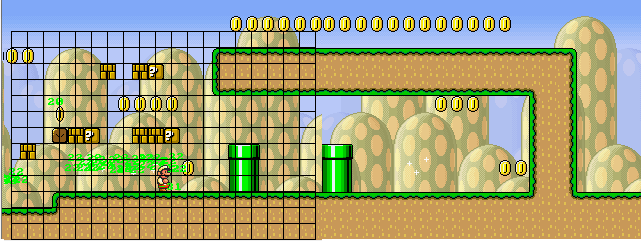
\includegraphics[width=.53\textwidth]{trapMatrix}&
			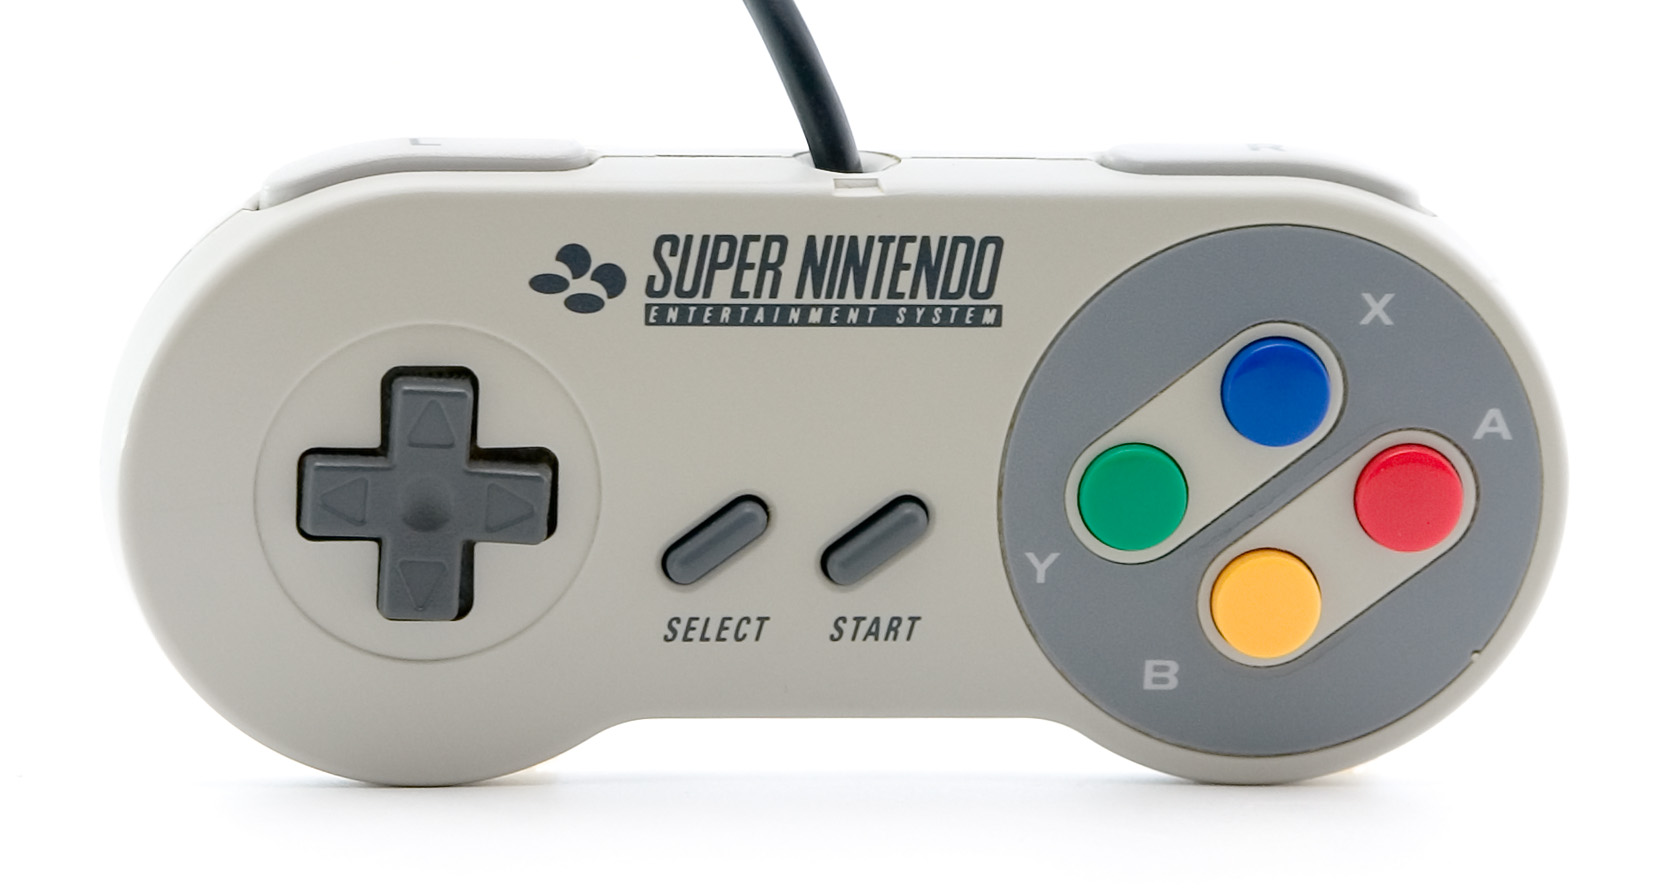
\includegraphics[width=.38\textwidth]{snesControl}\\
			\end{tabular}
		\end{center}
	\end{block}
	\vfill
\end{frame}

\begin{frame}{}
	\frametitle{Mario AI}
	\begin{block}{Navigation}
		\begin{itemize}
			\item Need to navigate through structural hazards;
			\item Dynamic path: blocks can be broken;
			\item Instant calculation of path through level:
			\begin{itemize}
				\item Use dynamically updated A* navigation.
			\end{itemize}
		\end{itemize}
	\end{block}
	\begin{block}{Reactiveness}
		\begin{itemize}
			\item Instant, reactive behaviour required;
			\item Too dynamic for online learning;
			\item Well encoded as condition-action associations:
			\begin{itemize}
				\item Evolve Behaviour Trees offline using Grammatical Evolution.
			\end{itemize}
		\end{itemize}
	\end{block}
	\vfill
\end{frame}

%%%%%%%%%%%%%%%%%%%%%%%%%%%%%%%%%%%%%%%%%%%%%%%%%%%%%%%%%%%%%%%%%%%%%%%%%%%%%%%
\section{A* for Navigation}
%%%%%%%%%%%%%%%%%%%%%%%%%%%%%%%%%%%%%%%%%%%%%%%%%%%%%%%%%%%%%%%%%%%%%%%%%%%%%%%

\begin{frame}{}
	\frametitle{Navigation: A*}
	\begin{block}{Graph creation}
		\begin{itemize}
			\item Map not available at start, must be built during navigation;
			\item Use discrete coordinate system to store tiled version of level;
			\item Identify nodes:
			\begin{itemize}
				\item Places where Mario can stand;
				\item Store extra information (such as what is over each node).
			\end{itemize}
		\end{itemize}
		\begin{center}
			\begin{tabular}{cc}
			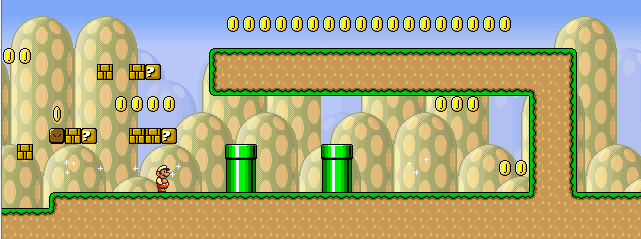
\includegraphics[width=.45\textwidth]{trap}&
			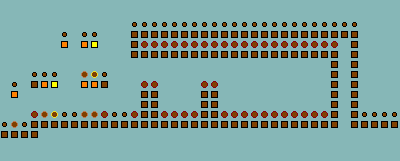
\includegraphics[width=.45\textwidth]{trapNodes}\\
			\end{tabular}
		\end{center}
	\end{block}
	\vfill
\end{frame}

\begin{frame}{}
	\frametitle{Navigation: A*}
	\begin{block}{Graph creation}
		\begin{itemize}
			\item Non-zenithal perspective: horizontal edges $\neq$ vertical edges;
			\item Different types of links:\\
			\begin{tabular}{ll}
				\textbf{A}: Walk links; & \textbf{D}: Faith jump links;\\
				\textbf{B}: Jump links; & \textbf{E}: Break jump links. \\
				\textbf{C}: Fall links;
			\end{tabular}
			\item Cost: Manhattan distance + modifier for jumps.
		\end{itemize}
		\begin{center}
			\begin{tabular}{cc}
			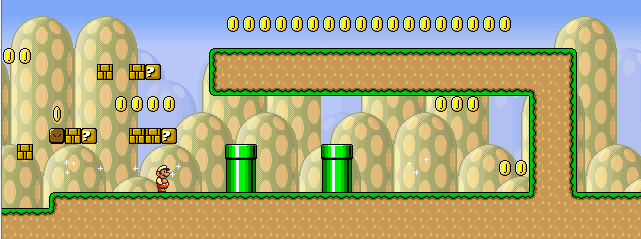
\includegraphics[width=.45\textwidth]{trap}&
			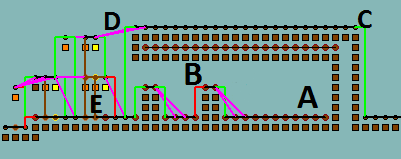
\includegraphics[width=.45\textwidth]{trapMapNoted}\\
			\end{tabular}
		\end{center}
	\end{block}
	\vfill
\end{frame}

%%%%%%%%%%%%%%%%%%%%%%%%%%%%%%%%%%%%%%%%%%%%%%%%%%%%%%%%%%%%%%%%%%%%%%%%%%%%%%%
\section{Behaviour Trees for Reactiveness}
%%%%%%%%%%%%%%%%%%%%%%%%%%%%%%%%%%%%%%%%%%%%%%%%%%%%%%%%%%%%%%%%%%%%%%%%%%%%%%%

\begin{frame}{}
	\frametitle{Reactiveness: Behaviour Trees}
	\begin{block}{Overview}
		\begin{itemize}
			\item Introduced as a means to specify system requirements;
			\item Lately used to encode game AI (\textit{Halo, Spore, Fa\c{c}ade, Defcon}).
		\end{itemize}
	\end{block}
	\begin{block}{AI Application}
		\begin{itemize}
			\item Hierarchically encode behaviours by decreasing order of complexity:
			$\star soldierBehaviour$\\
			\footnotesize{\ $\star attack$}\\
			\scriptsize{\ \ \ $\star aimingAlgorithm$}\\
			\tiny{\ \ \ \ \ \ $\star tracking$}\\
			\Tiny{\ \ \ \ \ \ \ \ \ \ldots}\\
			\Tiny{\ \ \ \ \ \ \ \ \ \ $\star playSprite$}
		\end{itemize}
	\end{block}
	\vfill
\end{frame}

\begin{frame}{}
	\frametitle{Behaviour Trees}
	\begin{block}{Components}
		\begin{itemize}
			\item \textit{Control Nodes}: \textbf{Sequence}, \textbf{Selector}, \textbf{Filter};
		\end{itemize}
	\begin{center}
		\begin{tabular}{ccc}
		
\includegraphics[width=.23\textwidth]{sequence}&
		
\includegraphics[width=.23\textwidth]{selector}&
		
\includegraphics[width=.048\textwidth]{filter}\\
		\end{tabular}
	\end{center}
		\begin{itemize}
			\item \textit{Leaf Nodes}: \textbf{Conditions}, \textbf{Actions}.
		\end{itemize}
	\end{block}
	\vfill
\end{frame}

\begin{frame}{}
	\frametitle{Behaviour Trees for Mario}
	\begin{block}{Integration}
		\begin{itemize}
			\item Synchronise Mario and BT execution:
			\begin{itemize}
				\item BT parsing resumes from previously reached point.
			\end{itemize}
			\item Provide nodes for evolution:
		\end{itemize}
		\begin{center}
		\scriptsize{\texttt{\begin{tabular}{|l|l|l|l|}
			\hline
			Filters		&	Conditions&	Actions&	Sub-trees\\
			\hline
			Loops		&	EnemyAhead&\textit{LRUDJF}&	JumpRightLong\\
			NON		&	UnderQuestion&RunRight	&	VerticalJump\\
			\ldots		&	\ldots	&GetPathToRightMostPosition&	\ldots\\
			\ldots		&	\ldots	&GetPathToClosestQuestion&	\ldots\\
			\hline
		\end{tabular}}}
		\end{center}
	\end{block}
	\vfill
\end{frame}

%%%%%%%%%%%%%%%%%%%%%%%%%%%%%%%%%%%%%%%%%%%%%%%%%%%%%%%%%%%%%%%%%%%%%%%%%%%%%%%
\section{Grammatical Evolution}
%%%%%%%%%%%%%%%%%%%%%%%%%%%%%%%%%%%%%%%%%%%%%%%%%%%%%%%%%%%%%%%%%%%%%%%%%%%%%%%

\begin{frame}{}
	\frametitle{Grammatical Evolution}
	\begin{block}{Key Characteristics}
		\begin{itemize}
			\item Numerical strings evolved by any search algorithm:
			\item Syntax of solutions specified by grammar.
		\end{itemize}
	\end{block}
	\begin{center}
		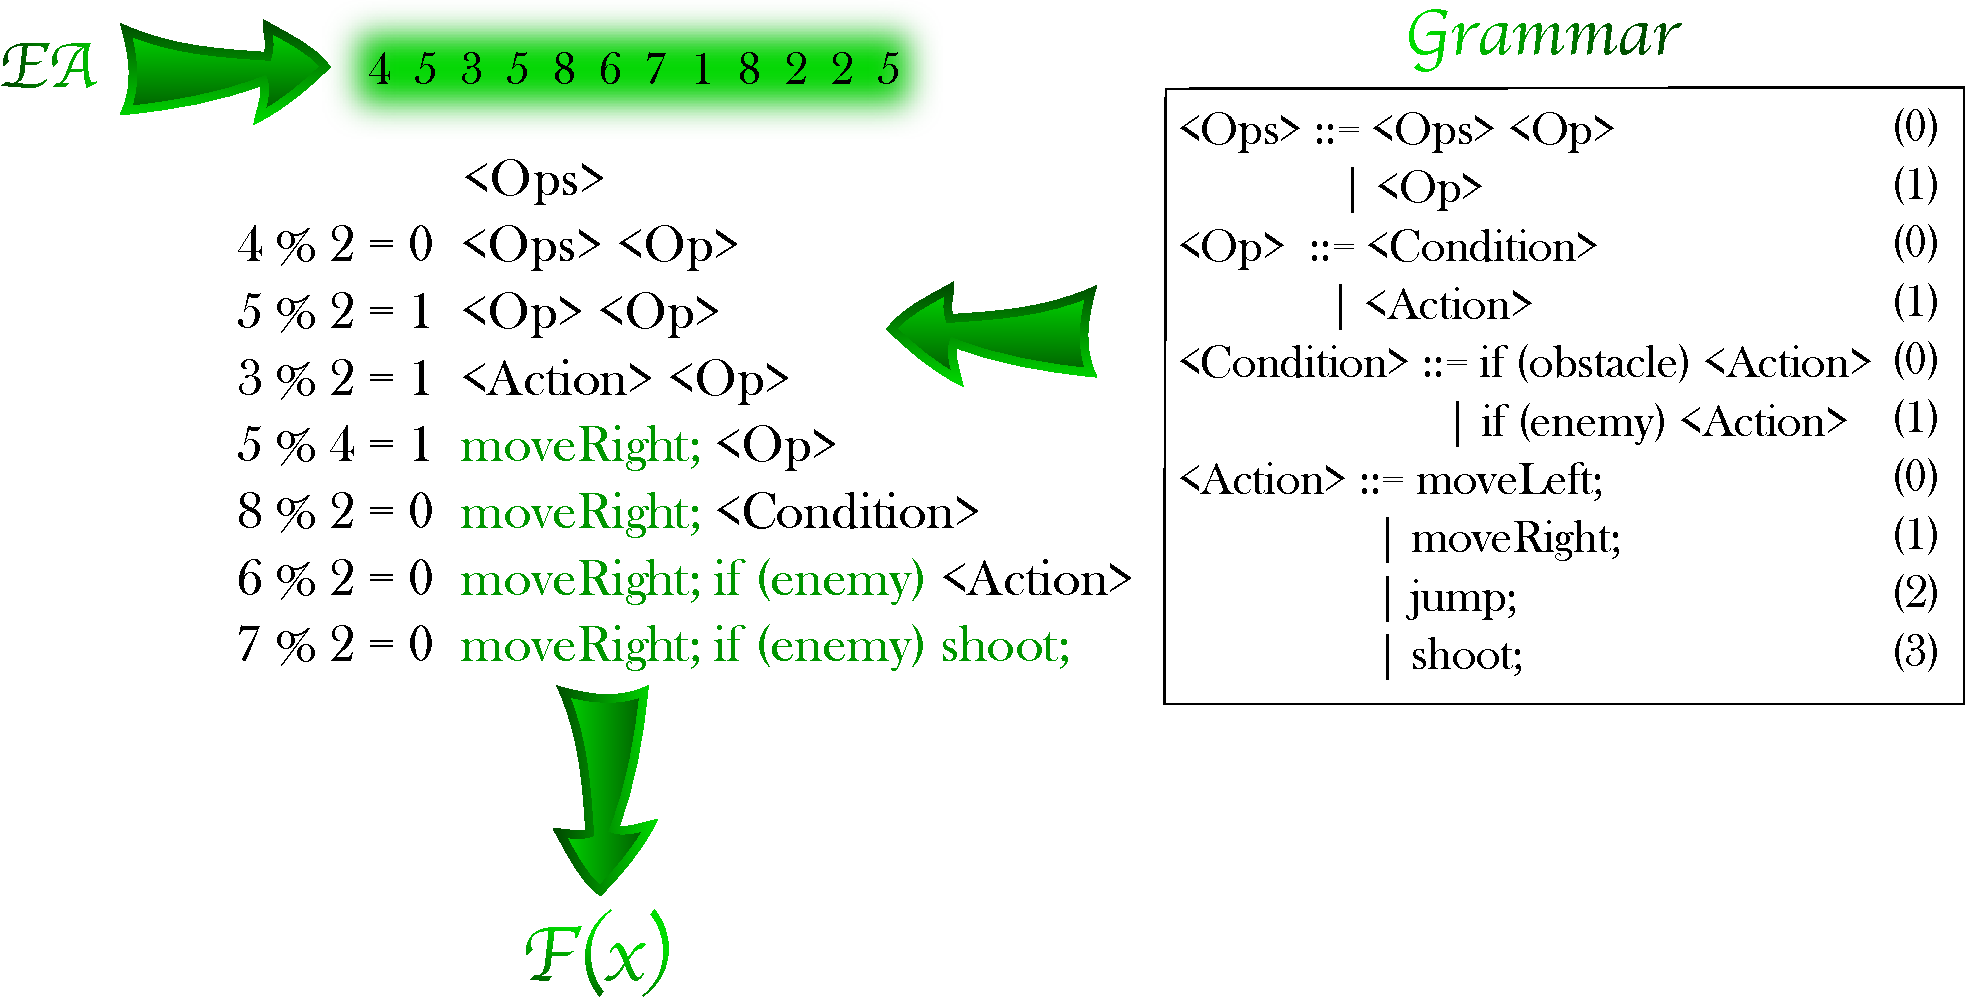
\includegraphics[width=.8\textwidth]{GEex.pdf}
	\end{center}
	\vfill
\end{frame}

%\begin{frame}{}
%	\frametitle{Grammatical Evolution}
%	\begin{center}
%		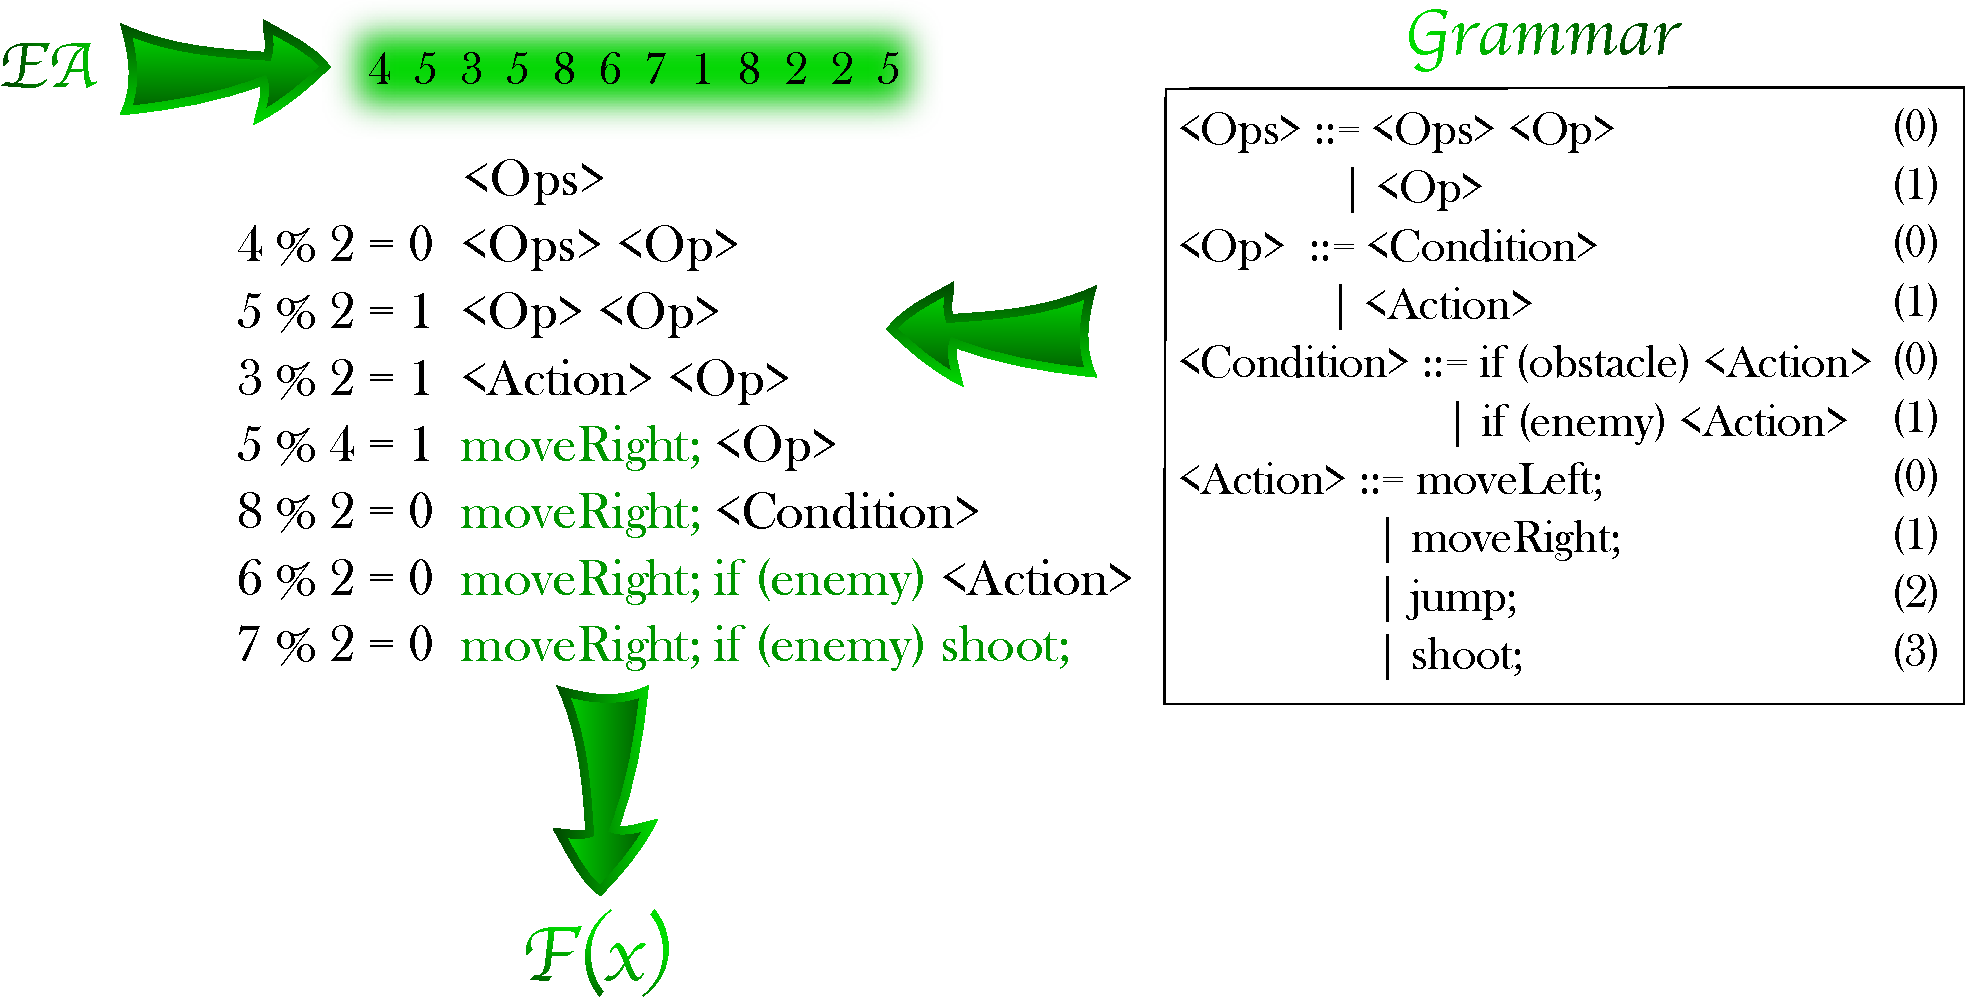
\includegraphics[width=1.0\textwidth]{GEex.pdf}
%	\end{center}
%	\vfill
%\end{frame}

\begin{frame}{}
	\frametitle{Grammatical Evolution}
	\begin{block}{Evolving Behaviour Trees}
		\begin{itemize}
			\item XML syntax specified through grammar;
			\item All conditions ($18$), actions ($15$), sub-trees ($14$) and filters ($4$);
			\item Limit syntax combinations through grammar (and-or trees).
		\end{itemize}
		\begin{center}
			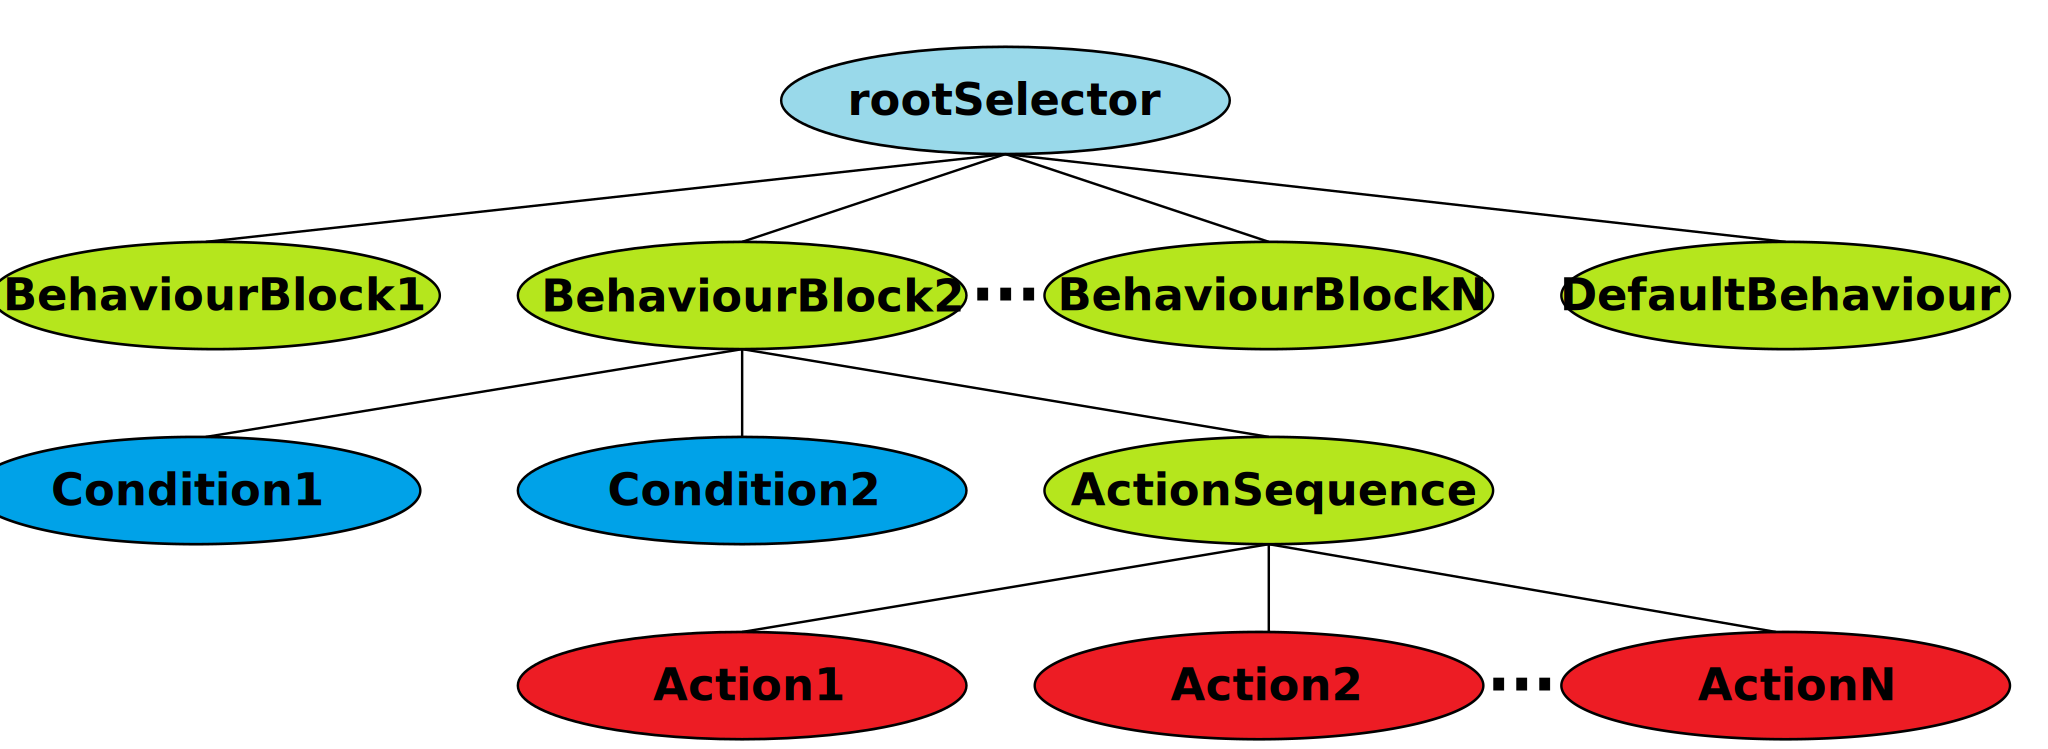
\includegraphics[width=.65\textwidth]{defaultTree}
		\end{center}
	\end{block}
	\vfill
\end{frame}

%%%%%%%%%%%%%%%%%%%%%%%%%%%%%%%%%%%%%%%%%%%%%%%%%%%%%%%%%%%%%%%%%%%%%%%%%%%%%%%
\section{Experiments and Results}
%%%%%%%%%%%%%%%%%%%%%%%%%%%%%%%%%%%%%%%%%%%%%%%%%%%%%%%%%%%%%%%%%%%%%%%%%%%%%%%

\begin{frame}
	\frametitle{Experiments}
	\begin{block}{Experimental Setup}
		\begin{center}
		\scriptsize{\begin{tabular}{|c|l|r|}
			\hline
			&Population Size & 500\\
			&Evaluations     & 125000\\
			%&Derivation-tree Depth (for initialisation) & 20\ldots 30\\
			%&Tail Ratio (for initialisation) & 50\%\\
			%GE&Selection Tournament Size & 1\%\\
			%&Elitism (for generational replacement) & 10\%\\
			GE&Marked 2-point Crossover Ratio & 50\%\\
			&Marked Swap Crossover Ratio & 50\%\\
			&Average Mutation Events per Individual & 1\\
			\hline
			\ \ Mario\ \ &Level Difficulties & 0 1 2 3 4 \\
			&Level Types & 0 1 \\
			%&Level Lengths & 320\\
			\hline
		\end{tabular}}
		\end{center}
	\end{block}
	\begin{block}{Generalisation Score}
		\begin{itemize}
			\item Measured on $360$ unseen levels:
			\begin{itemize}
				\item $20$ different map sets;
				\item $9$ level difficulties;
				\item $2$ level types.
			\end{itemize}
		\end{itemize}
	\end{block}
	\vfill
\end{frame}

\begin{frame}
	\frametitle{Experiments}
	\begin{block}{Generalisation Issues}
		\begin{itemize}
			\item Dynamic problem: controllers tested in unseen maps;
			\item Three approaches:
		\end{itemize}
		\begin{center}
			\scriptsize{\begin{tabular}{|l|c|c|c|}
				\cline{2-4}
				\multicolumn{1}{c|}{}& \textbf{Run1} & \textbf{Run5} & \textbf{Change1}\\
				\hline
				Map sets per evaluation& 1 & 5 & 1 \\
				\hline
				Change sets between evaluations & No & No & Yes \\
				\hline
			\end{tabular}}
		\end{center}
	\end{block}
	\vfill
\end{frame}

\begin{frame}
	\frametitle{Results}
	\begin{center}
		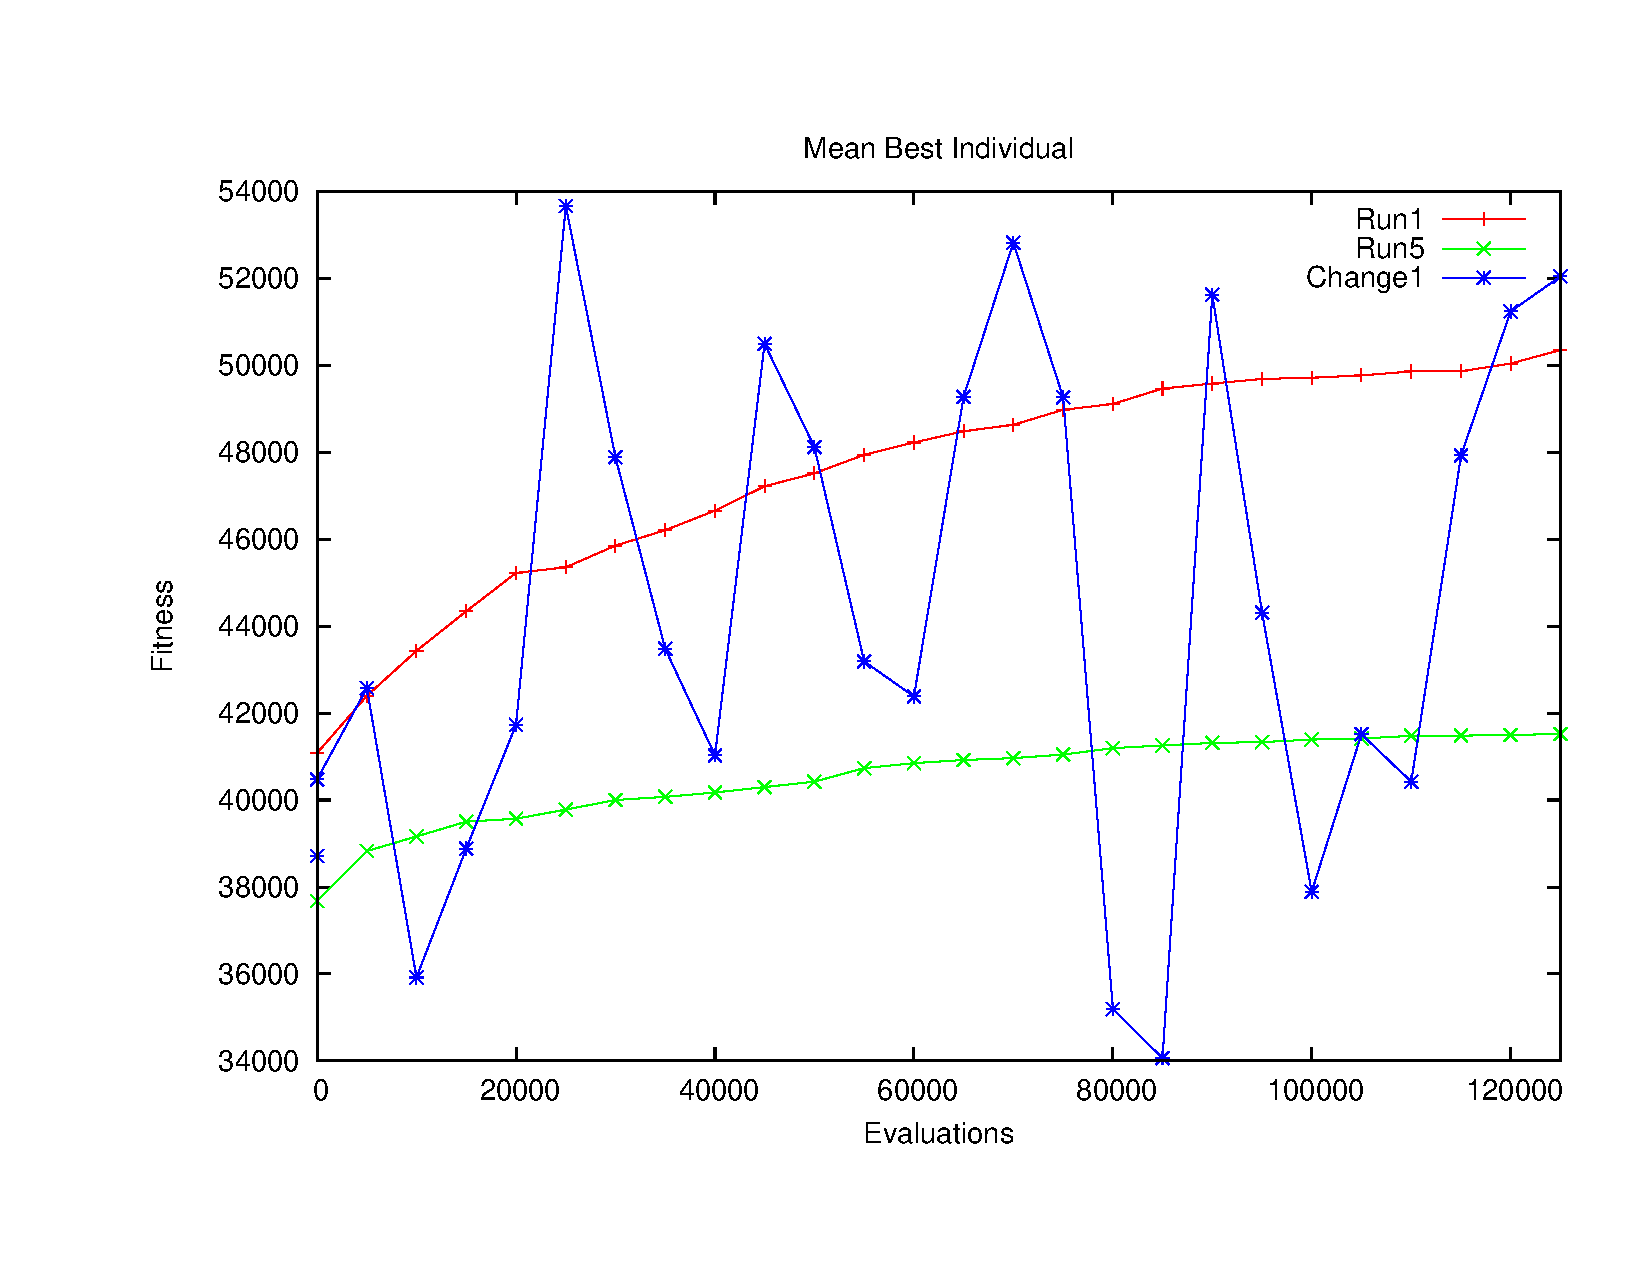
\includegraphics[width=.75\paperwidth]{mbi}
	\end{center}
	\vfill
\end{frame}

\begin{frame}
	\frametitle{Results}
	\begin{center}
		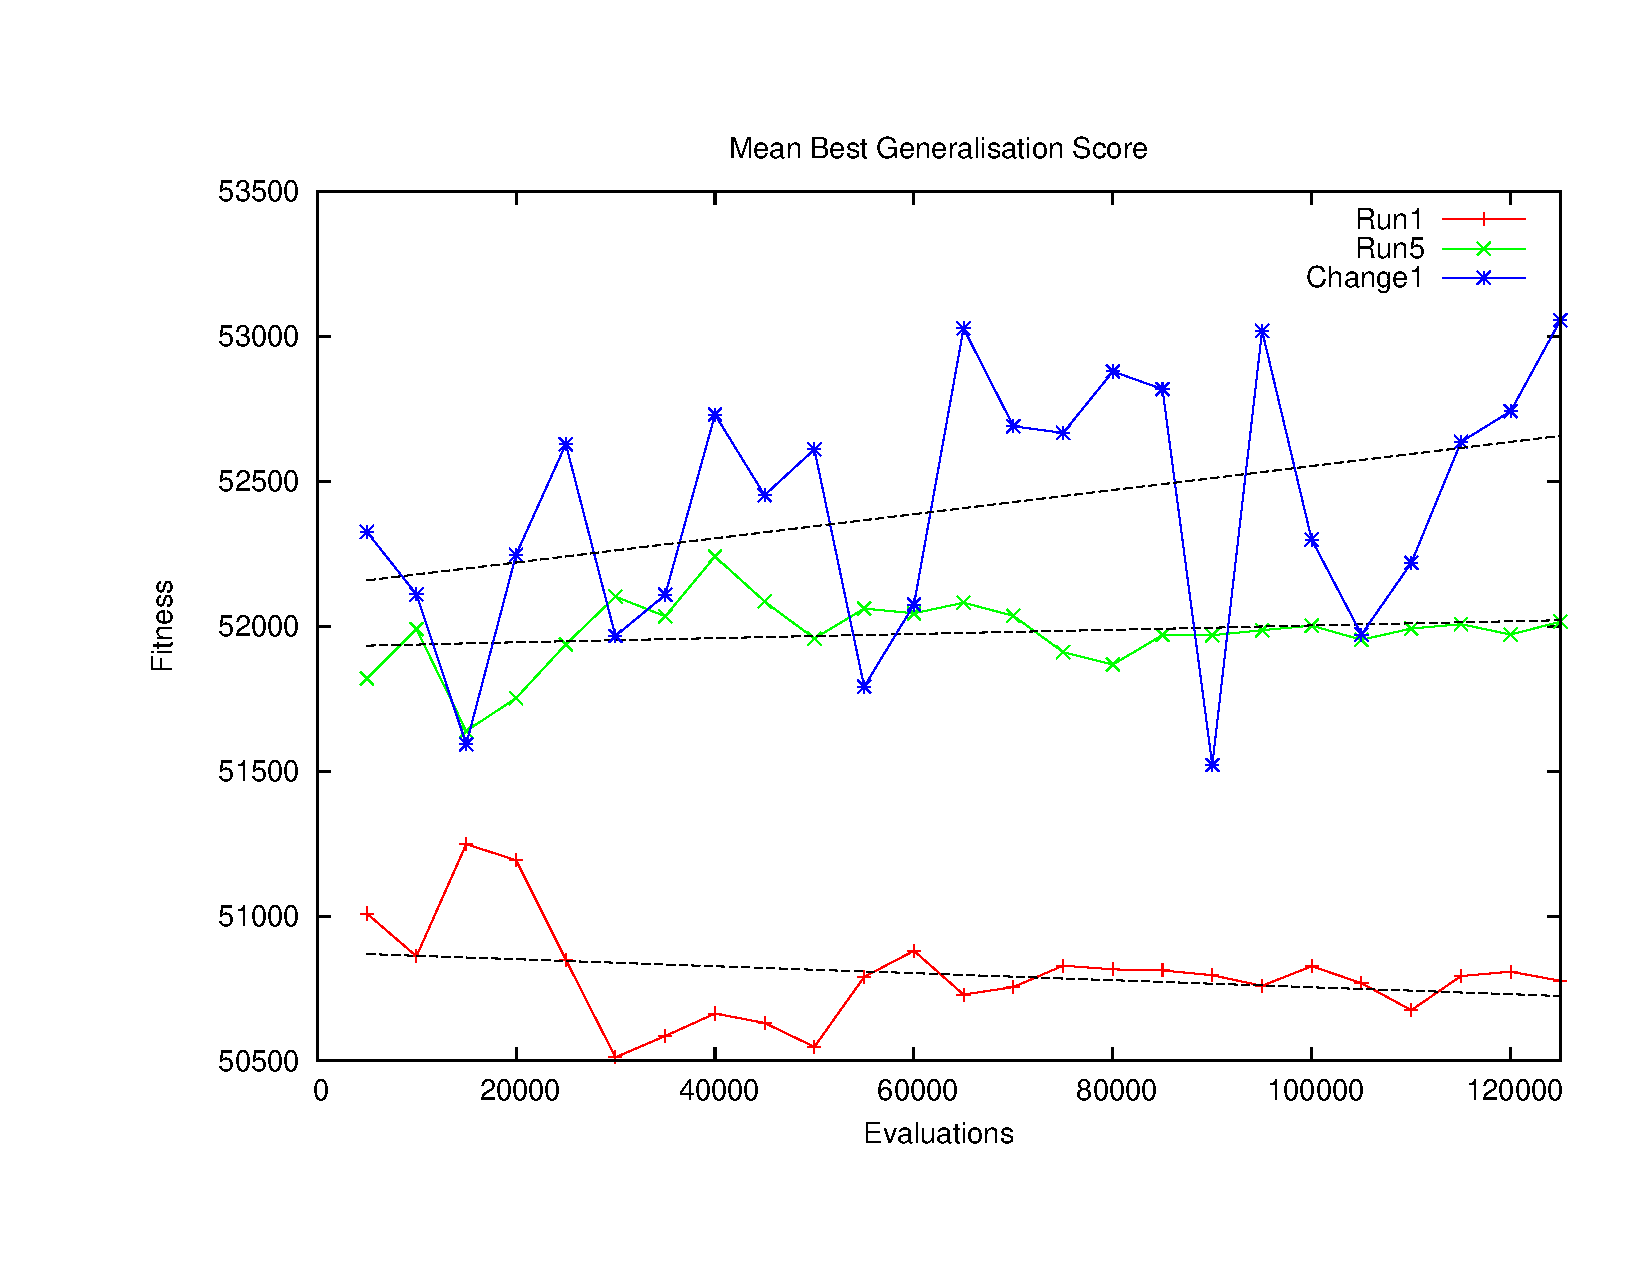
\includegraphics[width=.75\paperwidth]{mbg}
	\end{center}
	\vfill
\end{frame}


%%%%%%%%%%%%%%%%%%%%%%%%%%%%%%%%%%%%%%%%%%%%%%%%%%%%%%%%%%%%%%%%%%%%%%%%%%%%%%%
\section{Conclusions}
%%%%%%%%%%%%%%%%%%%%%%%%%%%%%%%%%%%%%%%%%%%%%%%%%%%%%%%%%%%%%%%%%%%%%%%%%%%%%%%

\begin{frame}
	\frametitle{Conclusions}
	\begin{block}{Navigation \& Reactiveness}
		\begin{itemize}
			\item Dynamic A* provides updated path following routines;
			\item Behaviour Tree routines enable fast-reacting behaviour;
			\item Grammatical Evolution combines both through evolution:
			\begin{itemize}
				\item Grammar facilitates syntax specification;
				\item Genetic operators exchange meaningful \textit{building-blocks}.
			\end{itemize}
		\end{itemize}
	\end{block}
	\begin{block}{Future Work}
		\begin{itemize}
			\item Improve generalisation performance:
			\begin{itemize}
				\item Training and generalisation tests;
				\item Sliding windows.
			\end{itemize}
		\end{itemize}
	\end{block}
	\vfill
\end{frame}

\begin{frame}
	\frametitle{Acknowledgements}
	\begin{itemize}
		\item SFI support grant number 08/IN.1/I868;
		\item A big \textbf{Thank You!} to all NCRA members.
	\end{itemize}
	\begin{center}
		
\includegraphics[width=.35\paperwidth]{SFI}
		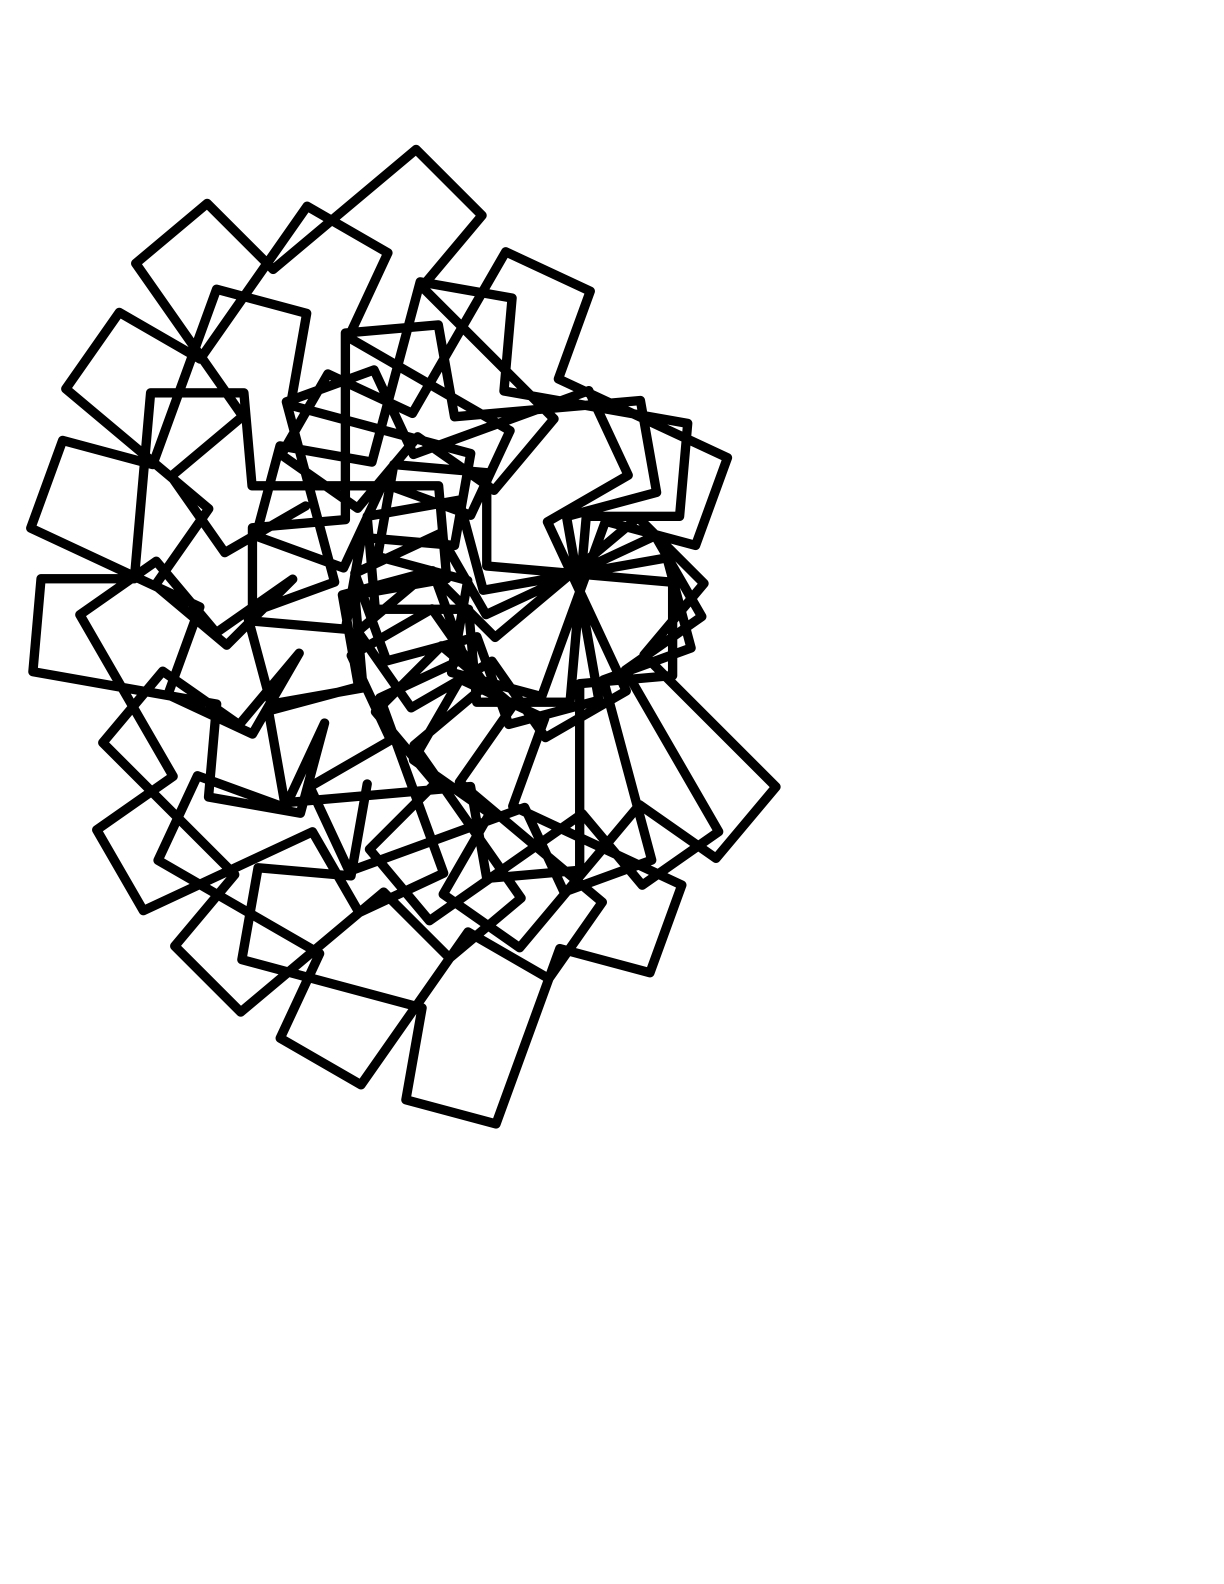
\includegraphics[width=.20\paperwidth]{ncralogo}
	\end{center}
\end{frame}


\end{document}

